
\PassOptionsToPackage{unicode}{hyperref}
\PassOptionsToPackage{hyphens}{url}
\PassOptionsToPackage{dvipsnames,svgnames,x11names}{xcolor}
%
\documentclass[
  11,
  ignorenonframetext,
  aspectratio=169,
  xcolor=table,
]{beamer}

\usepackage{pgfpages}
\setbeamertemplate{caption}[numbered]
\setbeamertemplate{caption label separator}{: }
\setbeamercolor{caption name}{fg=normal text.fg}
\setbeamertemplate{frametitle continuation}{}
\beamertemplatenavigationsymbolsempty

% Prevent slide breaks in the middle of a paragraph
\widowpenalties 1 10000
\raggedbottom
\usepackage{amsmath,amssymb}
\usepackage{booktabs}
\usepackage{lmodern}
\usepackage{iftex}
\ifPDFTeX
  \usepackage[T1]{fontenc}
  \usepackage[utf8]{inputenc}
  \usepackage{textcomp} % provide euro and other symbols
\else % if luatex or xetex
  \usepackage{unicode-math}
  \defaultfontfeatures{Scale=MatchLowercase}
  \defaultfontfeatures[\rmfamily]{Ligatures=TeX,Scale=1}
\fi
\usetheme[]{metropolis}
\usefonttheme{default}
% Use upquote if available, for straight quotes in verbatim environments
\IfFileExists{upquote.sty}{\usepackage{upquote}}{}
\IfFileExists{microtype.sty}{% use microtype if available
  \usepackage[]{microtype}
  \UseMicrotypeSet[protrusion]{basicmath} % disable protrusion for tt fonts
}{}
\makeatletter
\@ifundefined{KOMAClassName}{% if non-KOMA class
  \IfFileExists{parskip.sty}{%
    \usepackage{parskip}
  }{% else
    \setlength{\parindent}{0pt}
    \setlength{\parskip}{6pt plus 2pt minus 1pt}}
}{% if KOMA class
  \KOMAoptions{parskip=half}}
\makeatother
\usepackage{xcolor}
\newif\ifbibliography
\usepackage{graphicx}
\makeatletter
\def\maxwidth{\ifdim\Gin@nat@width>\linewidth\linewidth\else\Gin@nat@width\fi}
\def\maxheight{\ifdim\Gin@nat@height>\textheight\textheight\else\Gin@nat@height\fi}
\makeatother
% Scale images if necessary, so that they will not overflow the page
% margins by default, and it is still possible to overwrite the defaults
% using explicit options in \includegraphics[width, height, ...]{}
\setkeys{Gin}{width=\maxwidth,height=\maxheight,keepaspectratio}
% Set default figure placement to htbp
\makeatletter
\def\fps@figure{htbp}
\makeatother
\setlength{\emergencystretch}{3em} % prevent overfull lines
\providecommand{\tightlist}{%
  \setlength{\itemsep}{0pt}\setlength{\parskip}{0pt}}
\setcounter{secnumdepth}{-\maxdimen} % remove section numbering
\setbeamertemplate{section in toc}[round]
\setbeamerfont{section number projected}{size=\large}
\setbeamercolor{section number projected}{bg=red,fg=green}
\metroset{sectionpage=none}
\usefonttheme[onlymath]{serif}

\bibliographystyle{splncs04}
\usepackage[spanish]{babel}
\usepackage{subcaption}
\usepackage{multirow}
\usepackage{amsfonts}
\usepackage{bm}
\usepackage{amsmath}
\usepackage{booktabs}
\usepackage{algorithm2e}
\usepackage{algorithmicx}
\usepackage{colortbl}

\ifLuaTeX
  \usepackage{selnolig}  % disable illegal ligatures
\fi
\IfFileExists{bookmark.sty}{\usepackage{bookmark}}{\usepackage{hyperref}}
\IfFileExists{xurl.sty}{\usepackage{xurl}}{} % add URL line breaks if available
\urlstyle{same} % disable monospaced font for URLs
\hypersetup{
  pdftitle={Diseño Evolutivo de Redes Neuronales con Evolución Diferencial},
  pdfauthor={Alfredo Gutiérrez Alfaro},
  colorlinks=true,
  linkcolor={Maroon},
  filecolor={Maroon},
  citecolor={Blue},
  urlcolor={green},
  pdfcreator={LaTeX via pandoc}}

\title{Diseño Evolutivo de Redes Neuronales con Evolución Diferencial}
\author{Alfredo Gutiérrez Alfaro}
\date{\today}

\begin{document}
\frame{\titlepage}

\begin{frame}[shrink=5]
  \frametitle{Tabla de contenidos}
  \tableofcontents[hideallsubsections]
\end{frame}

\section{Introducción}
\begin{frame}{Introducción}
  \protect\hypertarget{introducciuxf3n}{}
  \begin{itemize}
    \item
          A la hora de implementar redes neuronales para resolver un problema
          requiere de personas expertas para diseñar la topología de la red y
          paramétros, entre otros elementos de diseño. \cite{lopez-vazquez-2019}
    \item
          Para resolver esta problemática del diseño, en la literatura se puede
          encontrar el uso de metaheuristicas bioinspiradas, como lo es el uso
          del Particle Swarm Optimization (PSO), Ant-Colony y la Evolución
          Diferencial. \cite{garro-2015,lopez-vazquez-2019,Alba-Cisneros2020}
  \end{itemize}
\end{frame}

\section{Objetivo}
\begin{frame}{Objetivo}
  \protect\hypertarget{objetivo}{}
  \begin{itemize}
    \item
          Implementar y analizar la evolución diferencial para el diseño de
          redes neuronales y cómo se desempeñan en las tareas de clasificación.
    \item
          Comparar resultados con una red neuronal ''tradicional'' entrenada con
          el descenso del gradiente
  \end{itemize}
\end{frame}

\section{Redes neuronales}
\begin{frame}{Redes Neuronales}
  \protect\hypertarget{redes-neuronales}{}
  \begin{columns}[T]
    \begin{column}{0.48\textwidth}
      Las redes neuronales son un modelo matemático que intentan replicar de
      cierta forma a las neuronas biológicas.

      \begin{equation}
        \sigma (\sum_{i=1}^m x_i w_i + b) = \sigma(x^T w + b) = \hat{y}
      \end{equation}
    \end{column}

    \begin{column}{0.48\textwidth}
      \begin{figure}
        \centering
        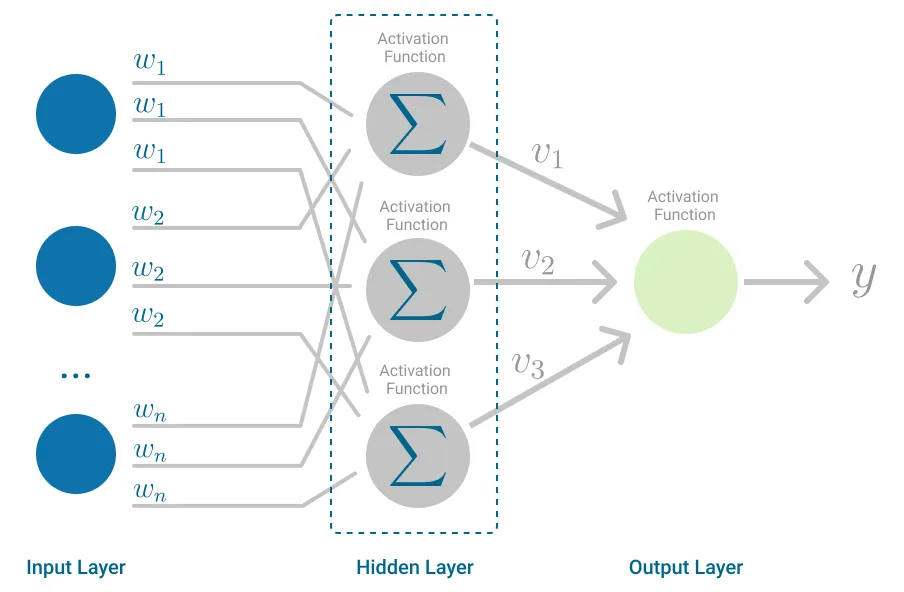
\includegraphics{images/network.png}
        \caption{Ejemplo red neuronal \cite{bento-2022}}
      \end{figure}
    \end{column}
  \end{columns}
\end{frame}

\subsection{Funciones de activación}
\begin{frame}[shrink=10]
  \frametitle{Redes neuronales}
  \protect\hypertarget{redes-neuronales-1}{}
  \begin{block}{Funciones de activación}
    \protect\hypertarget{funciones-de-activaciuxf3n}{}
    Las funciones de activación introducen no linealidad dentro de una red
    neuronal, lo que le permite a la red realizar representaciones más
    complejas de los datos.

    \begin{table}[]
      \begin{tabular}{|l|l|}
        \hline
        \textbf{Nombre} & \multicolumn{1}{c|}{\textbf{Función}}                                                 \\ \hline
        Sigmoid         & $\sigma(x) = \frac{1}{1 + e^{-x}}$                                                    \\ \hline
        Tanh            & $\tanh(x) = \frac{e^x - e^{-x}}{e^x + e^{-x}}$                                        \\ \hline
        Sinusoidal      & $\sin(x)$                                                                             \\ \hline
        Linear          & $f(x) = x$                                                                            \\ \hline
        Hard Limit      & $f(x) = \begin{cases} 1 & \text{si } x \geq 0 \\ 0 & \text{si } x < 0 \end{cases}$    \\ \hline
        ReLU            & $f(x) = \max(0, x)$                                                                   \\ \hline
        Leaky ReLU      & $f(x) = \begin{cases} 0.1x & \text{si } x < 0 \\ x & \text{si } x \geq 0 \end{cases}$ \\ \hline
      \end{tabular}
    \end{table}
  \end{block}
\end{frame}

\section{Aprendizaje evolutivo}
\begin{frame}{Aprendizaje evolutivo}
  \protect\hypertarget{aprendizaje-evolutivo}{}
  Los algoritmos evolutivos son un tipo de algoritmos de optimización
  heurísticos y aleatorizados, inspirados en la evolución natural. Simulan
  el proceso de evolución natural considerando dos factores clave: la
  reproducción variacional y la selección del más apto. \cite{zhou-2019}

  Los estructura básica de la mayoría de algoritmos evolutivos se puede
  resumir de la siguiente manera:

  \begin{enumerate}
    \item Generar un conjunto inicial de soluciones (llamado población).
    \item Reproducir nuevas soluciones basadas en la población actual, mediante procesos como el cruce y la mutación.
    \item Eliminar las peores soluciones de la población.
    \item Repetir desde el paso 2 hasta que se cumpla algún criterio de parada.
  \end{enumerate}
\end{frame}

\subsection{Evolución diferencial}
\begin{frame}{Evolución diferencial}
  \protect\hypertarget{evoluciuxf3n-diferencial}{}
  La evoluación diferencial es un algoritmo evolutivo que sirve para
  resolver problemas continuos. La ED utiliza una estrategia multiparental
  para generar posibles soluciones. El algoritmo se basa en la
  reproducción de uno o más individuos, reemplazando a los padres por
  hijos con mejor aptitud. \cite{du-2016}
\end{frame}

\subsection{Pseudocódigo}
\begin{frame}[shrink=10]
  \frametitle{Evolución diferencial}
  \protect\hypertarget{evoluciuxf3n-diferencial-1}{}
  \begin{block}{Pseudocódigo}
    \protect\hypertarget{pseudocuxf3digo}{}
    \begin{algorithm}[H]

      \SetAlgoLined
      \SetKwInOut{Input}{Input}
      \SetKwInOut{Output}{Output}

      \Input{Number of individuals NP}
      \Output{Optimized solution P}

      Generate $P = (x1, x2, ..., xNP)$\;

      \Repeat{stopping condition is satisfied}{
        \For{$i = 1 to NP$}{
          Compute a mutant vector vi\;
          Create ui by the crossover of vi and xi\;

          \If{$f(ui) < f(xi)$}{
            Insert ui into Q\;
          }
          \Else{
            Insert xi into Q\;
          }
        }
        P $\leftarrow$ Q\;
      }
    \end{algorithm}
  \end{block}
\end{frame}


\begin{frame}[shrink=10]
  \frametitle{Evolución diferencial}
  \protect\hypertarget{evoluciuxf3n-diferencial-1}{}
  \begin{block}{Pseudocódigo}
    \protect\hypertarget{pseudocuxf3digo}{}
    \begin{algorithm}[H]

      \SetAlgoLined
      \SetKwInOut{Input}{Input}
      \SetKwInOut{Output}{Output}

      \Input{Number of individuals NP}
      \Output{Optimized solution P}

      Generate $P = (x1, x2, ..., xNP)$\;

      \Repeat{stopping condition is satisfied}{
        \For{$i = 1 to NP$}{
          Compute a mutant vector vi\;
          Create ui by the crossover of vi and xi\;

          \If{$f(ui) < f(xi)$}{
            Insert ui into Q\;
          }
          \Else{
            Insert xi into Q\;
          }
        }
        P $\leftarrow$ Q\;
      }
    \end{algorithm}
  \end{block}
\end{frame}

\begin{frame}[shrink=10]
  \frametitle{Evolución diferencial}
  \protect\hypertarget{evoluciuxf3n-diferencial-1}{}
  \begin{block}{Pseudocódigo}
    \protect\hypertarget{pseudocuxf3digo}{}
    \begin{algorithm}[H]

      \SetAlgoLined
      \SetKwInOut{Input}{Input}
      \SetKwInOut{Output}{Output}

      \Input{Number of individuals NP}
      \Output{Optimized solution P}

      Generate $P = (x1, x2, ..., xNP)$\;

      \Repeat{stopping condition is satisfied}{
        \For{$i = 1 to NP$}{
          Compute a mutant vector vi\;
          Create ui by the crossover of vi and xi\;

          \If{$f(ui) < f(xi)$}{
            Insert ui into Q\;
          }
          \Else{
            Insert xi into Q\;
          }
        }
        P $\leftarrow$ Q\;
      }
    \end{algorithm}
  \end{block}
\end{frame}

\documentclass{beamer}
\usepackage{graphicx}

\usetheme{Warsaw}

\begin{document}

\begin{frame}[shrink=5]
  \frametitle{Evolución diferencial}
  \begin{columns}[T]
    \begin{column}{0.5\textwidth}
      \begin{block}{Pseudocódigo}
        \footnotesize
        \begin{algorithm}[H]
          \SetAlgoLined
          \SetKwInOut{Input}{Input}
          \SetKwInOut{Output}{Output}

          \Input{Number of individuals NP}
          \Output{Optimized solution P}

          Generate $P = (x1, x2, ..., xNP)$\;

          \Repeat{stopping condition is satisfied}{
            \For{$i = 1$ to $NP$}{
              Compute a mutant vector $v_i$\;
              Create $u_i$ by the crossover of $v_i$ and $x_i$\;

              \If{$f(u_i) < f(x_i)$}{
                Insert $u_i$ into $Q$\;
              }
              \Else{
                Insert $x_i$ into $Q$\;
              }
            }
            $P \leftarrow Q$\;
          }
        \end{algorithm}
      \end{block}
    \end{column}

    \begin{column}{0.5\textwidth}
      \begin{block}{Python Code}
        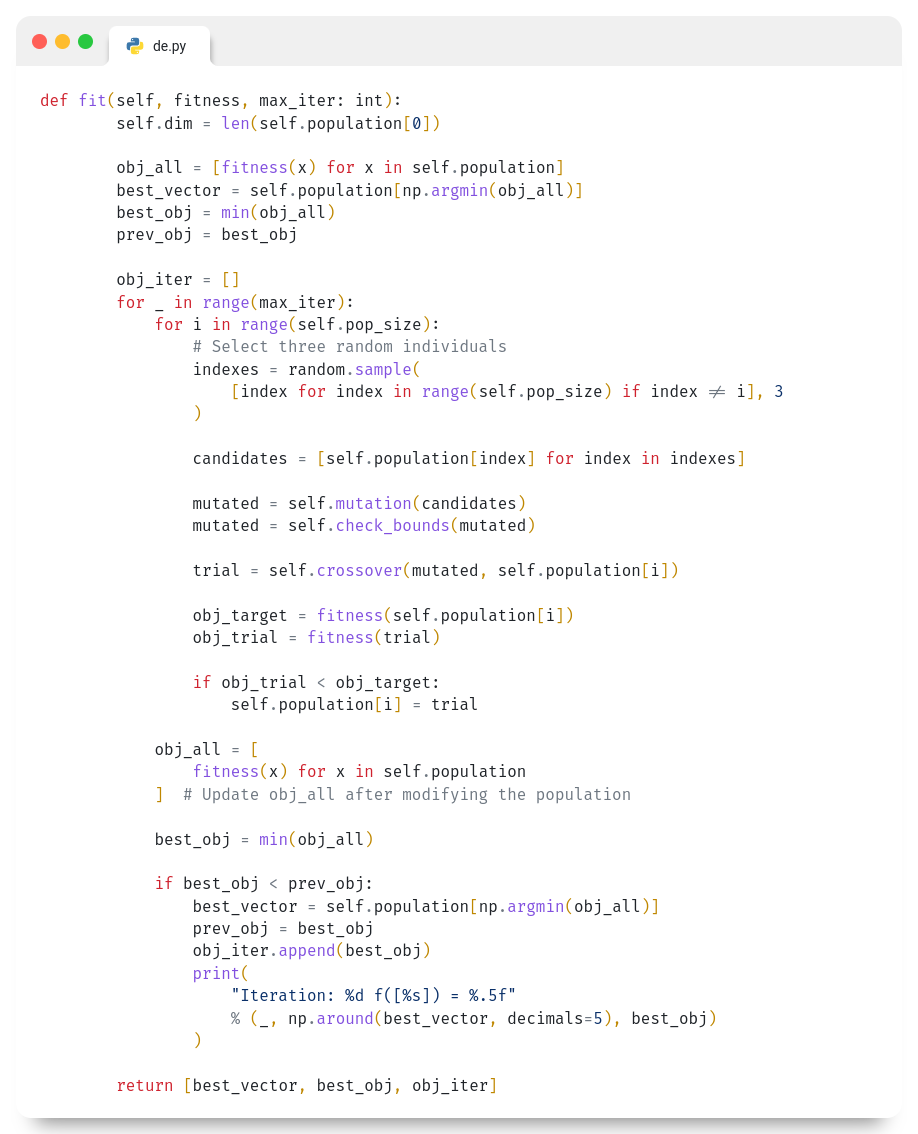
\includegraphics[width=\textwidth,height=0.9\textheight,keepaspectratio]{images/code.png}
      \end{block}
    \end{column}
  \end{columns}
\end{frame}


\section{Desarrollo}

\subsection{Representación del problema}
\begin{frame}{Representación del problema}
  \protect\hypertarget{representaciuxf3n-del-problema}{}
  \begin{block}{Metodología}
    \protect\hypertarget{metodologuxeda}{}
    Diseñar una red neuronal de tres capas con algorimos evolutivos
    (evolución diferencial) con un esquema de codificación directo
    \cite{garro-2015}, que tiene en consideración los siguientes elementos:

    \begin{enumerate}
      \tightlist
      \item
            Definir el número de neuronas en la capa oculta
      \item
            Establecer funciones de activación
      \item
            Generar conexiones sinapticas y pesos
    \end{enumerate}
  \end{block}
\end{frame}

\begin{frame}{Representación del problema}
  \protect\hypertarget{representaciuxf3n-del-problema-1}{}
  \begin{block}{}
    Definir el número total de neuronas en la red neuronal
    \protect\hypertarget{definir-el-nuxfamero-de-neuronas-en-la-capa-oculta}{}
    \begin{equation} \label{eq:total}
      Q = (M + N) + \frac{N+M}{2}
    \end{equation}

    Definir el número de neuronas en la capa de entrada
    \begin{equation} \label{eq:hidden}
      H = Q - (M + N)
    \end{equation}

    Obtener el tamaño de la dimensión del vector para representar el problema
    \begin{equation} \label{eq:dim}
      dim_d = [H * (N + 3)] + [M * (H + 3)]
    \end{equation}
  \end{block}
\end{frame}

\begin{frame}{Representación del problema}
  \protect\hypertarget{representaciuxf3n-del-problema-2}{}
  A continuación una muestra de cómo se representa la codificación para el
  diseño de las redes neuronales:

  \begin{figure}
    \centering
    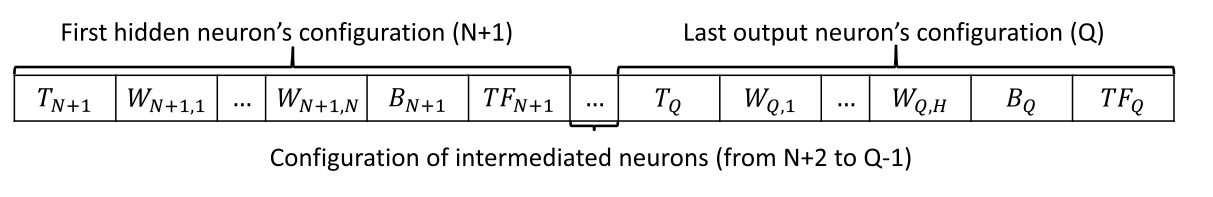
\includegraphics{images/representation.png}
    \caption{Esquema para representar los paramétros    \cite{Alba-Cisneros2020}}
  \end{figure}
\end{frame}

\section{Métricas}
\begin{frame}{Métricas}
  \protect\hypertarget{muxe9tricas}{}
  Para poder evaluar la red y utilizar una función a optimizar dentro de
  la evolución diferenciar se hará uso de la exactitud y el error de esta:

  \begin{equation}
    Exactitud = \frac{VP+VN}{VP+VN+FP+FN}
  \end{equation}

  \begin{equation}
    error = 1 - exactitud
  \end{equation}
\end{frame}

\section{Experimentos}
\begin{frame}{Experimentos}
  \protect\hypertarget{experimentos}{}
  Se utilizaron las ecuaciones {[}\ref{eq:total}, \ref{eq:hidden},
  \ref{eq:dim}{]} para generar las neuronas (arquitectura) de una red
  neuronal para dos conjuntos de datos diferentes: Iris Plant
  \cite{misc_iris_53} y Wine \cite{misc_wine_109}.

  Posteriormente esta red fue codificadas para ser utilizadas por la
  evolución diferencial y así obtener la topología de la red así como sus
  paramétros para después evaluar la red con la exactitud.
\end{frame}

\section{Resultados}
\begin{frame}
  \frametitle{Resultados}
  \begin{columns}[T]
    \begin{column}{0.5\textwidth}
      \begin{figure}
        \centering
        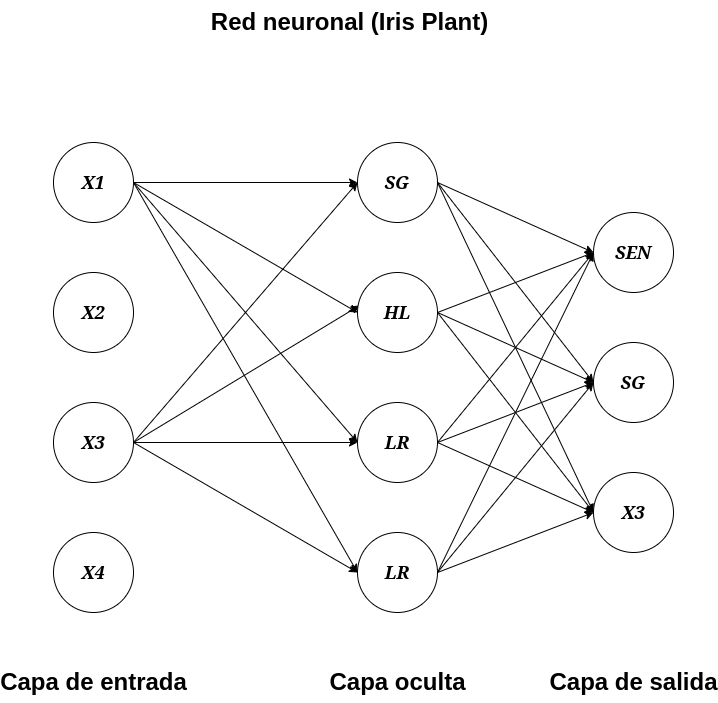
\includegraphics[width=\textwidth]{images/iris plant.drawio.png}
        \caption{Arquitectura para Iris}
      \end{figure}
    \end{column}

    \begin{column}{0.5\textwidth}
      \begin{figure}
        \centering
        \includegraphics[width=0.4\textwidth]{images/Diagrama sin título.drawio (1).png}
        \caption{Arquitectura para Wine}
      \end{figure}
    \end{column}
  \end{columns}
\end{frame}

\begin{frame}
  \frametitle{Resultados}
  \begin{columns}[T]
    \begin{column}{0.5\textwidth}
      \begin{figure}
        \centering
        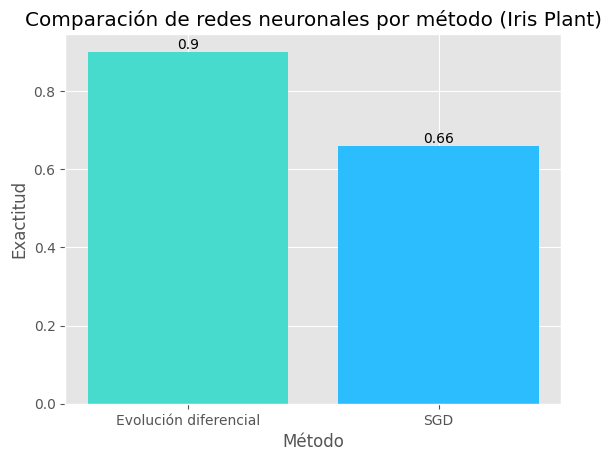
\includegraphics[width=\textwidth]{images/iris_comparision.png}
      \end{figure}
    \end{column}

    \begin{column}{0.5\textwidth}
      \begin{figure}
        \centering
        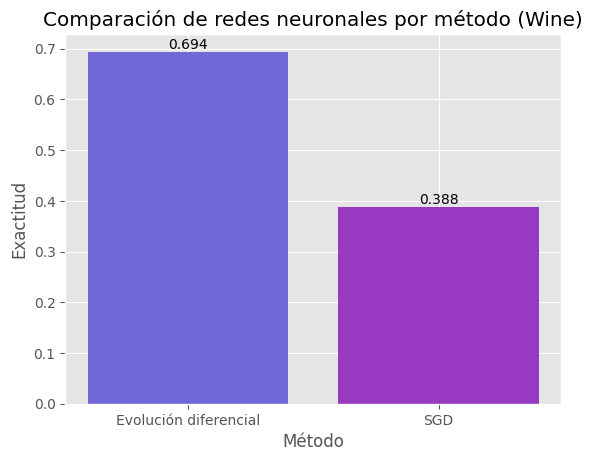
\includegraphics[width=\textwidth]{images/wine_comparision.png}
      \end{figure}
    \end{column}
  \end{columns}
\end{frame}
\begin{frame}{Conclusión}
  \protect\hypertarget{conclusiuxf3n}{}
  \begin{itemize}
    \item Las redes neuronales diseñadas por evolución diferencial llegan a tener mejores
          resultados que redes totalmente conectadas que utilizan el descenso del gradiente
    \item Las redes tienen mayor flexibilidad al ser diseñadas con una codificación directa
  \end{itemize}
\end{frame}

\begin{frame}[allowframebreaks]
  \frametitle{Referencias}
  \protect\hypertarget{referencias}{}
  \bibliographystyle{splncs04}
  \bibliography{gutierrez.bib}
\end{frame}

\end{document}
